\documentclass{standalone}
\usepackage{tikz}
\usetikzlibrary{patterns, positioning}

\begin{document}
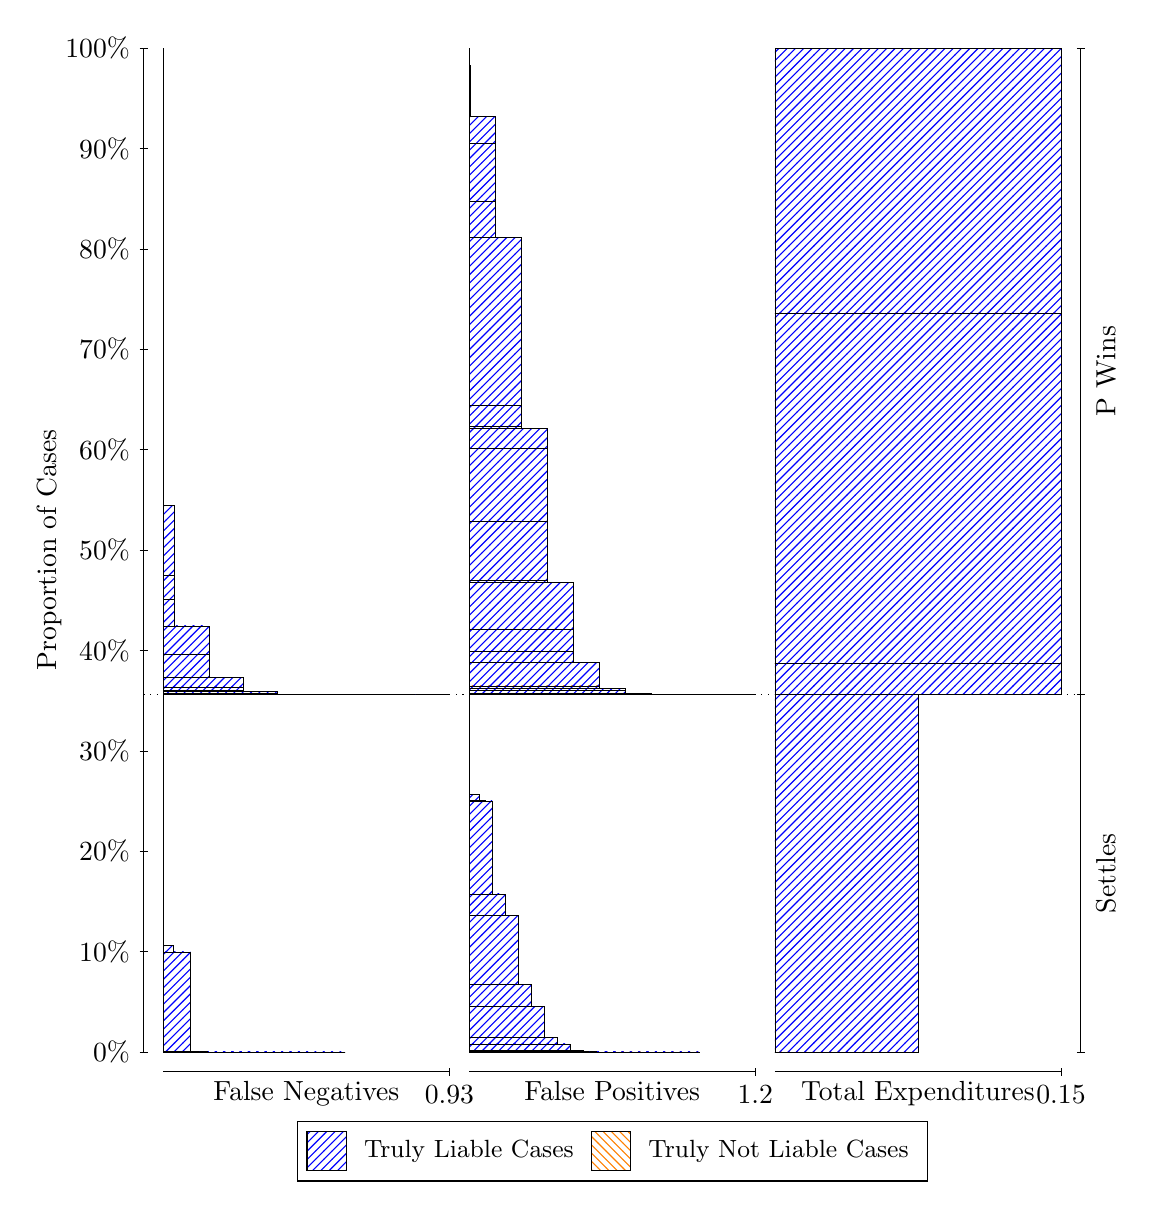
\begin{tikzpicture}
\draw[black, very thin] (1.5,1.75) -- (1.5,14.5);
\node[rotate=90, anchor=center] at (0.3, 8.125) {Proportion of Cases};
\draw[black, very thin] (1.45,1.75) -- (1.55,1.75);
\node[anchor=east] at (1.45, 1.75) {0\%};
\draw[black, very thin] (1.45,3.025) -- (1.55,3.025);
\node[anchor=east] at (1.45, 3.025) {10\%};
\draw[black, very thin] (1.45,4.3) -- (1.55,4.3);
\node[anchor=east] at (1.45, 4.3) {20\%};
\draw[black, very thin] (1.45,5.575) -- (1.55,5.575);
\node[anchor=east] at (1.45, 5.575) {30\%};
\draw[black, very thin] (1.45,6.85) -- (1.55,6.85);
\node[anchor=east] at (1.45, 6.85) {40\%};
\draw[black, very thin] (1.45,8.125) -- (1.55,8.125);
\node[anchor=east] at (1.45, 8.125) {50\%};
\draw[black, very thin] (1.45,9.4) -- (1.55,9.4);
\node[anchor=east] at (1.45, 9.4) {60\%};
\draw[black, very thin] (1.45,10.675) -- (1.55,10.675);
\node[anchor=east] at (1.45, 10.675) {70\%};
\draw[black, very thin] (1.45,11.95) -- (1.55,11.95);
\node[anchor=east] at (1.45, 11.95) {80\%};
\draw[black, very thin] (1.45,13.225) -- (1.55,13.225);
\node[anchor=east] at (1.45, 13.225) {90\%};
\draw[black, very thin] (1.45,14.5) -- (1.55,14.5);
\node[anchor=east] at (1.45, 14.5) {100\%};

\draw[black, very thin] (13.4,1.75) -- (13.4,14.5);
\draw[black, very thin] (13.35,1.75) -- (13.45,1.75);
\node[anchor=west] at (13.35, 1.75) {};
\draw[black, very thin] (13.35,6.2904) -- (13.45,6.2904);
\node[anchor=west] at (13.35, 6.2904) {};
\draw[black, very thin] (13.35,14.5) -- (13.45,14.5);
\node[anchor=west] at (13.35, 14.5) {};

\draw[black, very thin, pattern color=blue, pattern=north east lines] (1.75,1.75) rectangle (4.0577,1.75);
\draw[black, very thin, pattern color=blue, pattern=north east lines] (1.75,1.75) rectangle (3.6212,1.75);
\draw[black, very thin, pattern color=blue, pattern=north east lines] (1.75,1.75) rectangle (3.1848,1.75);
\draw[black, very thin, pattern color=blue, pattern=north east lines] (1.75,1.75) rectangle (3.0757,1.75);
\draw[black, very thin, pattern color=blue, pattern=north east lines] (1.75,1.75) rectangle (2.7483,1.7502);
\draw[black, very thin, pattern color=blue, pattern=north east lines] (1.75,1.7502) rectangle (2.6392,1.7502);
\draw[black, very thin, pattern color=blue, pattern=north east lines] (1.75,1.7502) rectangle (2.3119,1.7575);
\draw[black, very thin, pattern color=blue, pattern=north east lines] (1.75,1.7575) rectangle (2.2028,1.7575);
\draw[black, very thin, pattern color=blue, pattern=north east lines] (1.75,1.7575) rectangle (2.0937,3.0211);
\draw[black, very thin, pattern color=blue, pattern=north east lines] (1.75,3.0211) rectangle (1.8755,3.1001);
\draw[black, very thin, pattern color=blue, pattern=north east lines] (1.75,3.1001) rectangle (1.7664,3.1002);
\draw[black, very thin, pattern color=orange, pattern=north west lines] (1.75,3.1002) rectangle (1.75,3.1002);
\draw[black, very thin, pattern color=blue, pattern=north east lines] (1.75,3.1002) rectangle (1.75,6.2904);
\draw[black, very thin, pattern color=blue, pattern=north east lines] (1.75,6.2904) rectangle (5.3833,6.2904);
\draw[black, very thin, pattern color=blue, pattern=north east lines] (1.75,6.2904) rectangle (4.9469,6.2904);
\draw[black, very thin, pattern color=blue, pattern=north east lines] (1.75,6.2904) rectangle (4.5105,6.2904);
\draw[black, very thin, pattern color=blue, pattern=north east lines] (1.75,6.2904) rectangle (4.5105,6.2904);
\draw[black, very thin, pattern color=blue, pattern=north east lines] (1.75,6.2904) rectangle (4.074,6.2906);
\draw[black, very thin, pattern color=blue, pattern=north east lines] (1.75,6.2906) rectangle (4.074,6.2906);
\draw[black, very thin, pattern color=blue, pattern=north east lines] (1.75,6.2906) rectangle (3.6376,6.2906);
\draw[black, very thin, pattern color=blue, pattern=north east lines] (1.75,6.2906) rectangle (3.6376,6.2926);
\draw[black, very thin, pattern color=blue, pattern=north east lines] (1.75,6.2926) rectangle (3.6376,6.2938);
\draw[black, very thin, pattern color=blue, pattern=north east lines] (1.75,6.2938) rectangle (3.2012,6.3084);
\draw[black, very thin, pattern color=blue, pattern=north east lines] (1.75,6.3084) rectangle (3.2012,6.326);
\draw[black, very thin, pattern color=blue, pattern=north east lines] (1.75,6.326) rectangle (2.7647,6.3425);
\draw[black, very thin, pattern color=blue, pattern=north east lines] (1.75,6.3425) rectangle (2.7647,6.3875);
\draw[black, very thin, pattern color=blue, pattern=north east lines] (1.75,6.3875) rectangle (2.7647,6.509);
\draw[black, very thin, pattern color=blue, pattern=north east lines] (1.75,6.509) rectangle (2.3283,6.7992);
\draw[black, very thin, pattern color=blue, pattern=north east lines] (1.75,6.7992) rectangle (2.3283,7.16);
\draw[black, very thin, pattern color=blue, pattern=north east lines] (1.75,7.16) rectangle (1.8918,7.5011);
\draw[black, very thin, pattern color=blue, pattern=north east lines] (1.75,7.5011) rectangle (1.8918,7.7993);
\draw[black, very thin, pattern color=blue, pattern=north east lines] (1.75,7.7993) rectangle (1.8918,8.696);
\draw[black, very thin, pattern color=orange, pattern=north west lines] (1.75,8.696) rectangle (1.75,8.696);
\draw[black, very thin, pattern color=blue, pattern=north east lines] (1.75,8.696) rectangle (1.75,14.5);
\draw[black, very thin, pattern color=orange, pattern=north west lines] (5.6333,1.75) rectangle (8.5622,1.75);
\draw[black, very thin, pattern color=blue, pattern=north east lines] (5.6333,1.75) rectangle (8.5622,1.75);
\draw[black, very thin, pattern color=blue, pattern=north east lines] (5.6333,1.75) rectangle (8.2327,1.75);
\draw[black, very thin, pattern color=blue, pattern=north east lines] (5.6333,1.75) rectangle (7.9031,1.75);
\draw[black, very thin, pattern color=orange, pattern=north west lines] (5.6333,1.75) rectangle (7.8207,1.75);
\draw[black, very thin, pattern color=blue, pattern=north east lines] (5.6333,1.75) rectangle (7.8207,1.75);
\draw[black, very thin, pattern color=blue, pattern=north east lines] (5.6333,1.75) rectangle (7.5736,1.7502);
\draw[black, very thin, pattern color=blue, pattern=north east lines] (5.6333,1.7502) rectangle (7.4912,1.7502);
\draw[black, very thin, pattern color=blue, pattern=north east lines] (5.6333,1.7502) rectangle (7.244,1.7576);
\draw[black, very thin, pattern color=blue, pattern=north east lines] (5.6333,1.7576) rectangle (7.1616,1.7576);
\draw[black, very thin, pattern color=orange, pattern=north west lines] (5.6333,1.7576) rectangle (7.0793,1.7576);
\draw[black, very thin, pattern color=blue, pattern=north east lines] (5.6333,1.7576) rectangle (7.0793,1.7689);
\draw[black, very thin, pattern color=blue, pattern=north east lines] (5.6333,1.7689) rectangle (6.9145,1.8536);
\draw[black, very thin, pattern color=blue, pattern=north east lines] (5.6333,1.8536) rectangle (6.8321,1.8537);
\draw[black, very thin, pattern color=blue, pattern=north east lines] (5.6333,1.8537) rectangle (6.7497,1.9384);
\draw[black, very thin, pattern color=blue, pattern=north east lines] (5.6333,1.9384) rectangle (6.5849,2.3315);
\draw[black, very thin, pattern color=blue, pattern=north east lines] (5.6333,2.3315) rectangle (6.5025,2.332);
\draw[black, very thin, pattern color=blue, pattern=north east lines] (5.6333,2.332) rectangle (6.4201,2.605);
\draw[black, very thin, pattern color=blue, pattern=north east lines] (5.6333,2.605) rectangle (6.2554,3.4841);
\draw[black, very thin, pattern color=blue, pattern=north east lines] (5.6333,3.4841) rectangle (6.173,3.4847);
\draw[black, very thin, pattern color=blue, pattern=north east lines] (5.6333,3.4847) rectangle (6.0906,3.7565);
\draw[black, very thin, pattern color=blue, pattern=north east lines] (5.6333,3.7565) rectangle (5.9258,4.9402);
\draw[black, very thin, pattern color=blue, pattern=north east lines] (5.6333,4.9402) rectangle (5.8434,4.9403);
\draw[black, very thin, pattern color=blue, pattern=north east lines] (5.6333,4.9403) rectangle (5.761,5.0193);
\draw[black, very thin, pattern color=blue, pattern=north east lines] (5.6333,5.0193) rectangle (5.6333,6.2904);
\draw[black, very thin, pattern color=orange, pattern=north west lines] (5.6333,6.2904) rectangle (9.2667,6.2904);
\draw[black, very thin, pattern color=blue, pattern=north east lines] (5.6333,6.2904) rectangle (9.2667,6.2904);
\draw[black, very thin, pattern color=orange, pattern=north west lines] (5.6333,6.2904) rectangle (8.9371,6.2904);
\draw[black, very thin, pattern color=blue, pattern=north east lines] (5.6333,6.2904) rectangle (8.9371,6.2904);
\draw[black, very thin, pattern color=orange, pattern=north west lines] (5.6333,6.2904) rectangle (8.6076,6.2904);
\draw[black, very thin, pattern color=blue, pattern=north east lines] (5.6333,6.2904) rectangle (8.6076,6.2904);
\draw[black, very thin, pattern color=blue, pattern=north east lines] (5.6333,6.2904) rectangle (8.278,6.2906);
\draw[black, very thin, pattern color=blue, pattern=north east lines] (5.6333,6.2906) rectangle (8.278,6.2907);
\draw[black, very thin, pattern color=orange, pattern=north west lines] (5.6333,6.2907) rectangle (8.278,6.2907);
\draw[black, very thin, pattern color=blue, pattern=north east lines] (5.6333,6.2907) rectangle (8.278,6.2911);
\draw[black, very thin, pattern color=blue, pattern=north east lines] (5.6333,6.2911) rectangle (7.9485,6.2938);
\draw[black, very thin, pattern color=orange, pattern=north west lines] (5.6333,6.2938) rectangle (7.9485,6.2938);
\draw[black, very thin, pattern color=blue, pattern=north east lines] (5.6333,6.2938) rectangle (7.9485,6.2975);
\draw[black, very thin, pattern color=blue, pattern=north east lines] (5.6333,6.2975) rectangle (7.9485,6.2993);
\draw[black, very thin, pattern color=blue, pattern=north east lines] (5.6333,6.2993) rectangle (7.6189,6.3399);
\draw[black, very thin, pattern color=orange, pattern=north west lines] (5.6333,6.3399) rectangle (7.6189,6.3399);
\draw[black, very thin, pattern color=blue, pattern=north east lines] (5.6333,6.3399) rectangle (7.6189,6.3658);
\draw[black, very thin, pattern color=blue, pattern=north east lines] (5.6333,6.3658) rectangle (7.2893,6.3996);
\draw[black, very thin, pattern color=orange, pattern=north west lines] (5.6333,6.3996) rectangle (7.2893,6.3996);
\draw[black, very thin, pattern color=blue, pattern=north east lines] (5.6333,6.3996) rectangle (7.2893,6.698);
\draw[black, very thin, pattern color=blue, pattern=north east lines] (5.6333,6.698) rectangle (6.9598,6.8428);
\draw[black, very thin, pattern color=blue, pattern=north east lines] (5.6333,6.8428) rectangle (6.9598,7.1119);
\draw[black, very thin, pattern color=orange, pattern=north west lines] (5.6333,7.1119) rectangle (6.9598,7.1119);
\draw[black, very thin, pattern color=blue, pattern=north east lines] (5.6333,7.1119) rectangle (6.9598,7.714);
\draw[black, very thin, pattern color=blue, pattern=north east lines] (5.6333,7.714) rectangle (6.6302,7.7368);
\draw[black, very thin, pattern color=blue, pattern=north east lines] (5.6333,7.7368) rectangle (6.6302,8.4848);
\draw[black, very thin, pattern color=orange, pattern=north west lines] (5.6333,8.4848) rectangle (6.6302,8.4848);
\draw[black, very thin, pattern color=blue, pattern=north east lines] (5.6333,8.4848) rectangle (6.6302,9.4189);
\draw[black, very thin, pattern color=blue, pattern=north east lines] (5.6333,9.4189) rectangle (6.6302,9.6685);
\draw[black, very thin, pattern color=blue, pattern=north east lines] (5.6333,9.6685) rectangle (6.3007,9.7016);
\draw[black, very thin, pattern color=blue, pattern=north east lines] (5.6333,9.7016) rectangle (6.3007,9.966);
\draw[black, very thin, pattern color=orange, pattern=north west lines] (5.6333,9.966) rectangle (6.3007,9.966);
\draw[black, very thin, pattern color=blue, pattern=north east lines] (5.6333,9.966) rectangle (6.3007,12.094);
\draw[black, very thin, pattern color=blue, pattern=north east lines] (5.6333,12.094) rectangle (5.9711,12.56);
\draw[black, very thin, pattern color=blue, pattern=north east lines] (5.6333,12.56) rectangle (5.9711,13.293);
\draw[black, very thin, pattern color=blue, pattern=north east lines] (5.6333,13.293) rectangle (5.9711,13.63);
\draw[black, very thin, pattern color=blue, pattern=north east lines] (5.6333,13.63) rectangle (5.6416,14.281);
\draw[black, very thin, pattern color=blue, pattern=north east lines] (5.6333,14.281) rectangle (5.6333,14.5);
\draw[black, very thin, pattern color=orange, pattern=north west lines] (9.5167,1.75) rectangle (11.333,1.75);
\draw[black, very thin, pattern color=blue, pattern=north east lines] (9.5167,1.75) rectangle (11.333,6.2904);
\draw[black, very thin, pattern color=orange, pattern=north west lines] (9.5167,6.2904) rectangle (13.15,6.2904);
\draw[black, very thin, pattern color=blue, pattern=north east lines] (9.5167,6.2904) rectangle (13.15,6.6844);
\draw[black, very thin, pattern color=orange, pattern=north west lines] (9.5167,6.6844) rectangle (13.15,6.6844);
\draw[black, very thin, pattern color=blue, pattern=north east lines] (9.5167,6.6844) rectangle (13.15,11.136);
\draw[black, very thin, pattern color=orange, pattern=north west lines] (9.5167,11.136) rectangle (13.15,11.136);
\draw[black, very thin, pattern color=blue, pattern=north east lines] (9.5167,11.136) rectangle (13.15,14.5);
\draw[black, dotted] (1.5,6.2904) -- (13.4,6.2904);
\draw[black, very thin] (1.75,1.5) -- (5.3833,1.5);
\node[anchor=north] at (3.5667, 1.5) {False Negatives};
\draw[black, very thin] (5.3833,1.45) -- (5.3833,1.55);
\node[anchor=north] at (5.3833, 1.45) {0.93};

\draw[black, very thin] (5.6333,1.5) -- (9.2667,1.5);
\node[anchor=north] at (7.45, 1.5) {False Positives};
\draw[black, very thin] (9.2667,1.45) -- (9.2667,1.55);
\node[anchor=north] at (9.2667, 1.45) {1.2};

\draw[black, very thin] (9.5167,1.5) -- (13.15,1.5);
\node[anchor=north] at (11.333, 1.5) {Total Expenditures};
\draw[black, very thin] (13.15,1.45) -- (13.15,1.55);
\node[anchor=north] at (13.15, 1.45) {0.15};

\node[black, centered, rotate=90] at (13.72, 4.0202) {Settles};
\node[black, centered, rotate=90] at (13.72, 10.395) {P Wins};

\draw (7.449999999999999,1.5) node[draw=none] (baseCoordinate) {};
\begin{scope}[align=center]
        \matrix[scale=0.5, draw=black, below=0.5cm of baseCoordinate, nodes={draw}, column sep=0.1cm]{
            \node[rectangle, draw, minimum width=0.5cm, minimum height=0.5cm, pattern=north east lines, pattern color=blue] {}; &
            \node[draw=none, font=\small] (B) {Truly Liable Cases}; &
            \node[rectangle, draw, minimum width=0.5cm, minimum height=0.5cm, pattern=north west lines, pattern color=orange] {}; &
            \node[draw=none, font=\small] (B) {Truly Not Liable Cases}; \\
            };
\end{scope}

\end{tikzpicture}
\end{document}